\hypertarget{Node_8h}{
\section{Node.h File Reference}
\label{Node_8h}\index{Node.h@{Node.h}}
}


This graph shows which files directly or indirectly include this file:\begin{figure}[H]
\begin{center}
\leavevmode
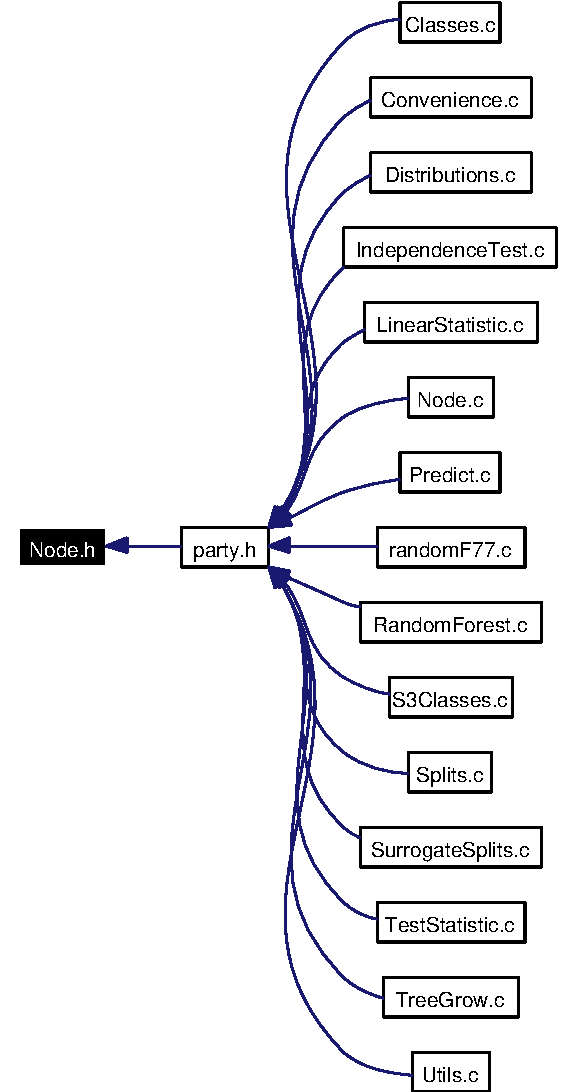
\includegraphics[width=157pt]{Node_8h__dep__incl}
\end{center}
\end{figure}
\subsection*{Functions}
\begin{CompactItemize}
\item 
void \hyperlink{Node_8h_0ed8b15b2c14ec9f1f1585d6288a38e2}{C\_\-Node} (SEXP node, SEXP learnsample, SEXP weights, SEXP fitmem, SEXP controls, int TERMINAL)
\end{CompactItemize}


\subsection{Function Documentation}
\hypertarget{Node_8h_0ed8b15b2c14ec9f1f1585d6288a38e2}{
\index{Node.h@{Node.h}!C_Node@{C\_\-Node}}
\index{C_Node@{C\_\-Node}!Node.h@{Node.h}}
\subsubsection[C\_\-Node]{\setlength{\rightskip}{0pt plus 5cm}void C\_\-Node (SEXP {\em node}, SEXP {\em learnsample}, SEXP {\em weights}, SEXP {\em fitmem}, SEXP {\em controls}, int {\em TERMINAL})}}
\label{Node_8h_0ed8b15b2c14ec9f1f1585d6288a38e2}


The main function for all node computations \begin{Desc}
\item[Parameters:]
\begin{description}
\item[{\em node}]an initialized node (an S3 object!) \item[{\em learnsample}]an object of class `Learning\-Sample' \item[{\em weights}]case weights \item[{\em fitmem}]an object of class `Tree\-Fit\-Memory' \item[{\em controls}]an object of class `Tree\-Control' \item[{\em TERMINAL}]logical indicating if this node will be a terminal node \end{description}
\end{Desc}


Definition at line 48 of file Node.c.

References C\_\-Global\-Test(), C\_\-init\_\-nominalsplit(), C\_\-init\_\-orderedsplit(), C\_\-max(), C\_\-prediction(), C\_\-split(), C\_\-splitcategorical(), C\_\-standardize(), C\_\-whichmax(), get\_\-dimension(), get\_\-gtctrl(), get\_\-levels(), get\_\-mincriterion(), get\_\-minsplit(), get\_\-ninputs(), get\_\-nobs(), get\_\-ordering(), get\_\-predict\_\-trafo(), get\_\-savesplitstats(), get\_\-splitctrl(), get\_\-splitstatistics(), get\_\-test\_\-trafo(), get\_\-tgctrl(), get\_\-tol(), get\_\-transformation(), get\_\-varctrl(), get\_\-variable(), get\_\-varmemory(), get\_\-weights(), has\_\-missings(), is\_\-nominal(), ncol(), PL2\_\-covariance\-Sym, PL2\_\-expcovinf\-Sym, PL2\_\-expectation\-Sym, PL2\_\-inputs\-Sym, PL2\_\-linearstatistic\-Sym, PL2\_\-linexpcov2sample\-Sym, PL2\_\-responses\-Sym, PL2\_\-sumweights\-Sym, S3\_\-SUMWEIGHTS, S3get\_\-criterion(), S3get\_\-maxcriterion(), S3get\_\-prediction(), S3get\_\-primarysplit(), S3get\_\-splitpoint(), S3get\_\-splitstatistics(), S3get\_\-table(), S3get\_\-teststat(), and S3set\_\-variable\-ID().

Referenced by C\_\-Tree\-Grow(), and R\_\-Node().

Here is the call graph for this function:\begin{figure}[H]
\begin{center}
\leavevmode
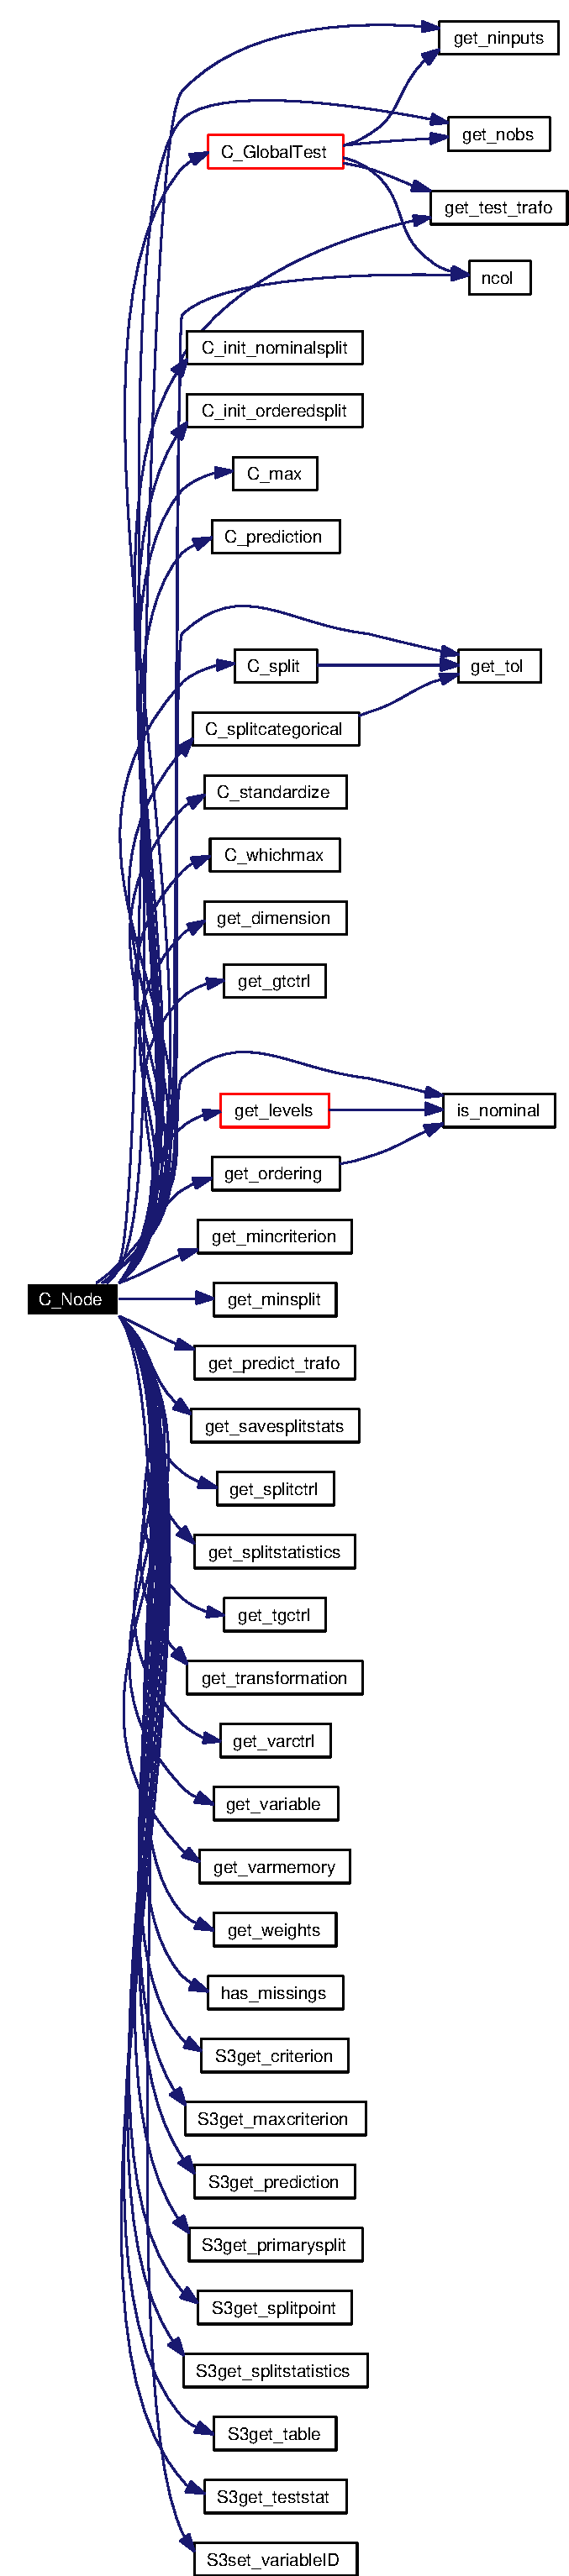
\includegraphics[width=180pt]{Node_8h_0ed8b15b2c14ec9f1f1585d6288a38e2_cgraph}
\end{center}
\end{figure}
